\textbf{\underline{OZ 8 - LC- en  RLC-circuits - Oefening 2:}}
\vspace{0.5cm}

Een spoel met $820$ windingen heeft een weerstand van $24,0 \ \Omega$, en wordt geplaatst rond een solenoïde met $12500$ windingen van $7.00$ cm lang. Zowel de spoel als de solenoïde hebben een doorsnede van oppervlakte $1.00\cdot10^{-4} \ \text{m}^2$.

\vspace{0.3cm}
\begin{minipage}{.66\textwidth}
    \begin{enumerate}[(a)]
        \item 
            Hoe lang duurt het voordat de stroom door de solenoïde $63,2\%$ van zijn maximale waarde bereikt?
        \item 
            Bepaal de gemiddelde tegen-emf veroorzaakt door de zelfinductie van de solenoïde tijdens dit tijdsinterval,
        \item 
            de gemiddelde snelheid van verandering van het magnetische flux door de spoel tijdens dit tijdsinterval,
        \item 
            en de grootte van de gemiddelde geïnduceerde stroom in de spoel.
    \end{enumerate}
\end{minipage}
\begin{minipage}{.3\textwidth}
    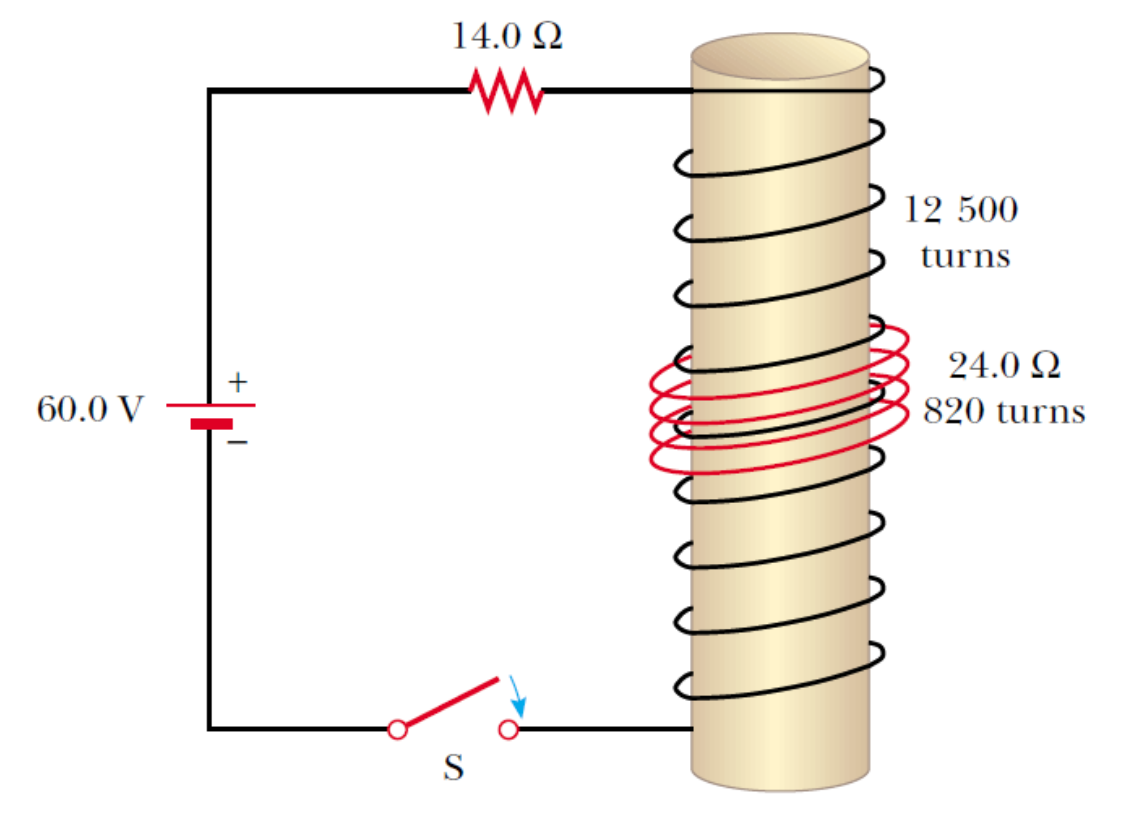
\includegraphics[scale = 0.3]{oz08/resources/Oz8Oef2.png}
\end{minipage}

\begin{enumerate}[(a)]
    \item 
        \begin{description}[labelwidth=1.5cm, leftmargin=!]
            \item[Geg. :]   
            \item[Gevr. :] 
            \item[Opl. :]   
        \end{description}
    \item 
        \begin{description}[labelwidth=1.5cm, leftmargin=!]
            \item[Geg. :]   
            \item[Gevr. :] 
            \item[Opl. :]   
        \end{description}
    \item 
        \begin{description}[labelwidth=1.5cm, leftmargin=!]
            \item[Geg. :]   
            \item[Gevr. :] 
            \item[Opl. :]   
        \end{description}
    \item 
        \begin{description}[labelwidth=1.5cm, leftmargin=!]
            \item[Geg. :]   
            \item[Gevr. :] 
            \item[Opl. :]   
        \end{description}
\end{enumerate}

\vspace{1cm}